\subsection{Variational Tree Walk}

\subsubsection{Microbiota dataset}

As we look into the microbiota data, one must a major phylogenetic architecture to describe various levels of precision in the microbiota composition.
Indeed, such phylogenetic structure can be represented as a tree as on the following figure:
\begin{figure}[H]
    \center
    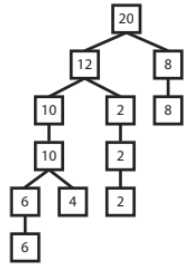
\includegraphics[scale=1]{images/abundance_tree_phylogenetic}
    \caption{Phylogenetic tree example with abundance data (in the nodes) at each layer of the tree.
    Each node represents a bacterium specie at a given precision layer in the tree. From \cite{microbiome_deeplearning_research}.}
    \label{fig:phylogenetic_tree}
\end{figure}

Such structure can not be used directly in a machine learning system since it's not a vectorizable representation.
Hence, we first suggest to transform the tree in a matrix to image structure as in the following example:
\begin{figure}[H]
    \center
    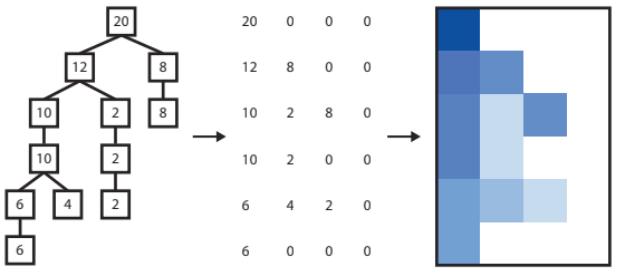
\includegraphics[scale=1]{images/tree_to_image}
    \caption{Phylogenetic tree to image representation:
    opacity of the pixel relates to the abundance of the species at the given level of precision (normalized between 0 and 1).
    From \cite{microbiome_deeplearning_research}.}
    \label{fig:phylogenetic_tree_to_img}
\end{figure}

Sadly this image representation does not convey the link between the species abundance given by the edges of the tree.
As a result, we suggest to find a hidden variable $Z$ that uses the adjacent matrix of the tree, to find a way to go through the image
as on the PixelCNN approach.
Such approach, in addition to use the adjacency of the tree graph, would then learn an interesting trajectory to compute the correlation between the abundance data.
The next section offers the mathematical framework of the proposed idea.

\subsubsection{Framework and optimization objectives}

\subsubsection{EM approach}

In first approximation, we would like to use the EM algorithm to try to compute the following latent model:
\begin{itemize}
    \item We assume that we have $n$ individuals
    \item The maximum size of a phylogenetic tree is $S$, and the maximum amount of unique species at a given level is $U$.
    \item $X_i$ is the abundance matrix of the individual $i$ (image of size $S \times U$) , which is observed.
    \item $T_i$ is the adjacent matrix of the phylogenetic tree of individual $i$, of size $S \times S$, which is observed.
    \item $Z_i$ is a hidden random walk over the tree $T_i$ (discrete vector, permutation of $(1, \dots, S)$).
          For a given random walk process over the tree, we denote by $N_{Z}$ the amount of possible generations ($N_Z \leq S!$).
          Hence, $p_{\gamma}(Z_i = z | T_i)$ is a known distribution defined by the random walk process.
    \item Taking inspiration from the PixelCNN, our model should learn the distribution $p_{\omega}(X_i | Z_i, T_i)$ as a CNN/RNN that is masked following $Z_i$.
          We also assume that conditionally to $Z_i$, this distribution is independent from the adjacent matrix: $p_{\omega}(X_i | Z_i, T_i) = p_{\omega}(X_i | Z_i)$.
\end{itemize}

Since we observe $\{T_i\}_{1 \leq i \leq n}$ phylogenetic trees, one can compute the empirical distribution of the edges of the graph denoted by $p_{T}$.
The computation of the empirical distribution is done by summing all the adjacent matrices $\{T_i\}_{1 \leq i \leq n}$ and dividing it by $n$:
$$
\bar{T} = \frac{1}{n} \sum_{i=1}^n T_i
$$
Then for any observed tree $t_i$, one can sum the edges probability in $\bar{T}$ and divide it by the amount of edges of the tree to obtain $\mathbb{P}(T = t_i)$. \\

Recall from the EM context that we aim at maximizing
$$
Q(\widehat{\theta}, \theta) = \mathbb{E}_{p_{\widehat{\theta}(Z|X,T)}}[\log p_{\theta}(X, Z, T) | X,T]
$$
Hence, we start with the \textbf{expectation} step and try to evaluate $p_{\widehat{\theta}(Z|X,T)}$:
$$
\begin{align}
    p_{\widehat{\theta}}(Z_i|X_i,T_i) = \tau_{ik} &= \log p_{\widehat{\theta}}(Z_i | T_i, X_i) \\
                                &= \log \frac{p(T_i) p_{\widehat{\theta}}(Z_i | T_i) p_{\widehat{\theta}}(X_i | Z_i, T_i)}{\sum_{j=1}^{N_Z} p(T_i) p_{\widehat{\theta}}(Z_i=z_j | T_i) p_{\widehat{\theta}}(X_i | Z_i=z_j, T_i)} \\
                                &= \log \frac{p_{\widehat{\theta}}(Z_i | T_i) p_{\widehat{\theta}}(X_i | Z_i)}{\sum_{j=1}^{N_Z} p_{\widehat{\theta}}(Z_i=z_j | T_i) p_{\widehat{\theta}}(X_i | Z_i=z_j)}
\end{align}
$$
Even though all terms seems computable and explicit here, the summation over $N_Z$ can be very large depending on the complexity of the random walk process we pick.
As a result, we will propose a variational approach to overcome this issue in the next section. \\

As it is right now, one could easily compute the \textbf{maximization} step for $Q(\widehat{\theta}, \theta)$ over $\theta = (\gamma, \omega)$, as it is now explicit:
$$
Q(\widehat{\theta}, \theta) = \sum_{i=1}^n (\log p(T_i) + \log p_{\gamma}(Z_i | T_i) + \log p_{\omega}(X_i | Z_i)) \tau_{ik}
$$

\subsubsection{Variational approach}

In this second approach, we aim at giving variational algorithm to compute a lower bound to the true objective.
To that end, since it can not be computed directly, we propose an estimate of $\p_{\theta}(Z|X,T) = q_{\Phi}(Z|X,T)$.
Recall then the ELBO explicited in the VAE general framework:
$$
\log p_{\theta}(X) = \underbrace{\mathbb{E}_{q_{\Phi}(Z|X,T)}\left[ \log \frac{p_{\theta}(X,Z,T)}{q_{\Phi}(Z|X,T)} \right]}_{ELBO(\Phi, \theta)} + D_{KL}[q_{\Phi}(Z|X,T) \Vert p_{\theta}(Z|X,T)]
$$
Such ELBO can be rewritten as:
$$
\begin{align}
    ELBO(\Phi, \theta) &= \mathbb{E}_{q_{\Phi}(Z|X,T)}[\log p_{\theta}(X,Z,T)] - \mathbb{E}_{q_{\Phi}(Z|X,T)}[\log q_{\Phi}(Z|X,T)] \\
                        &= \mathbb{E}_{q_{\Phi}(Z|X,T)}[\log p_{\theta}(X|Z,T)] - \mathbb{E}_{q_{\Phi}(Z|X,T)}\left[ \log \frac{q_{\Phi}(Z|X,T)}{p_{\gamma}(Z,T)} \right] \\
                        &= \mathbb{E}_{q_{\Phi}(Z|X,T)}[\log p_{\theta}(X|Z)] - D_{KL}[q_{\Phi}(Z|X,T) \Vert p_{\gamma}(Z|T)] + \log p(T)
\end{align}
$$

Taking inspiration from the VQ-VAE architecture, one might introduce a continuous primary variable $Z_i^e(T_i)$ following a gaussian distribution for instance,
and project it onto a finite space of random walks to obtain $Z_i^q(T_i)$.
As a result, $q_{\Phi}(Z_i|X_i,T_i) = \delta_{\{Z_i = Z_i^q\}}$, leading to the following objective:
$$
\begin{align}
    ELBO(\Phi, \theta) &= \sum_{i=1}^n \log p_{\omega}(X_i | Z_i^q(T_i)) - \log \frac{q_{\Phi}(Z_i^q(T_i) | X_i)}{p_{\gamma}(Z_i^q (T_i) | T_i)} \\
                        &= \sum_{i=1}^n \log p_{\omega}(X_i | Z_i^q(T_i)) + \log p_{\gamma}(Z_i^q (T_i) | T_i)
\end{align}
$$